\documentclass{VUMIFInfKursinis}
\usepackage{algorithmicx}
\usepackage{algorithm}
\usepackage{algpseudocode}
\usepackage{amsfonts}
\usepackage{amsmath}
\usepackage{bm}
\usepackage{color}
\usepackage{hyperref}  % Nuorodų aktyvavimas
\usepackage{url}

\usepackage{subcaption} % For subfigures
\usepackage{enumitem} % For 1.1 numbering in lists
\setlist[enumerate]{label*=\arabic*.}
\usepackage{multicol}
\usepackage{graphicx}
\usepackage[table,xcdraw]{xcolor}  % For table colors


\usepackage[font=small,labelfont=bf]{caption} 
\captionsetup[figure]{position=bottom}

% For code samples
\usepackage{listings}

\definecolor{dkgreen}{rgb}{0,0.6,0}
\definecolor{gray}{rgb}{0.5,0.5,0.5}
\definecolor{mauve}{rgb}{0.58,0,0.82}

\lstset{frame=tb,
  language=Python,
  aboveskip=3mm,
  belowskip=3mm,
  showstringspaces=false,
  columns=flexible,
  basicstyle={\scriptsize\ttfamily},
  numbers=left,
  numberstyle=\tiny\color{gray},
  keywordstyle=\color{blue},
  commentstyle=\color{dkgreen},
  stringstyle=\color{mauve},
  breaklines=true,
  breakatwhitespace=true,
  tabsize=4,
  keepspaces=true
}


% Titulinio aprašas
\university{Vilniaus universitetas}
\faculty{Matematikos ir informatikos fakultetas}
\department{Informatikos katedra}
\papertype{Kursinis projektinis darbas}
\title{Dokomentų klasterizacija}
\titleineng{Document clustering}
\status{4 kurso 1 grupės studentas}
\author{Dominykas Ablingis}
\supervisor{Prof., Dr. Rimantas Kybartas}
\date{Vilnius \\ \the\year}

% Nustatymai
\bibliography{bibliografija} 

%My macros

\newcommand{\ltang}[2]{#1 (angl.\  \textit{#2}) }
\newcommand{\BigO}[1]{$\mathcal{O}(#1)$}

\begin{document}

\maketitle
\tableofcontents

\sectionnonum{Įvadas}

Šio darbo tikslas yra aprašyti lietuviškų tekstinių dokumentų parengimo
klasterizavimui žingsnius, išanalizuoti naudotus metodus ir rezultatus,
gautus taikant skirtingus klasterizavimo algoritmus, bei įvertinti
suklasterizuotų tekstinių dokumentų kokybę.

\subsection*{Duomenų analizės eiga}

Klasterizavimas tėra vienas iš žingsnių tekstinių duomenų analizės
procese. Tekstinių duomenų analizės procesą galime suskirstyti į keletą
žingsnių \cite{fayyad1996data}:

\begin{enumerate}
\item
	\ltang{Probleminės srities nustatymas}{problem domain}. 
\item
	\ltang{Duomenų surinkimas}{data collection}.
\item
	\ltang{Duomenų tvarkymas ir apdorojimas}{cleaning and
	preprocessing}\footnote{3 ir 4-tas žingsniai gali būti apibrėžti kaip
		\ltang{požymių pasirinkimas}{feature selection}. Svarbu
		atrinkti požymius, kurie yra esminiai atskiriant objektus ir juose
		būtų konkreti informacija užduočiai atlikti, tuo pačiu stengiantis
		palikti kuo mažiau perteklinės informacijos ir neprarasti svarbios
		informacijos.}.
\item
	\ltang{Duomenų supaprastinimas ir transformavimas}{reduction and
	projection}.
\item
	\ltang{Duomenų analizavimas}{data analysis}.

  \begin{enumerate}
  \item
  	\ltang{Panašumo matas}{proximity measure}
  \item
  	\ltang{Panašumo matas}{proximity measure}
  \end{enumerate}
\item
  \ltang{Rezultatų validavimas / įvertinimas }{ validation of
results}
\item
  \ltang{Rezultatų interpretavimas}{ interpretacion of results} 
\item
  Rezultatų panaudojimas. 
\end{enumerate}

Ankstesniame darbe aprašiau 2, 3, 4 ir 6 žingsnius, šiame ir
įsigilinsiu į juos.










\section{Tekstinio duomenų rinkinio parengimas}

Rengiant tekstinį duomenų rinkinį klasterizavimui, 
\ltang{teksto paruošimo}{text preprocessing} metu tekstą iš patogios žmogui ar
kitoms programoms formos verčiame į formą tinkamą duomenų analizei. Tam
tekstinį dokumentą pirmiausia reikia papildomai apdoroti, t. y. jį
supaprastinti, pašalinti nereikalingus ir nereikšmingus žodžius,
stengiantis neprarasti mūsų uždavinio sprendimui vertingos informacijos.
Po to, tekstinius duomenis reikia paversti į skaitmeninius, kad galėtume
taikyti klasterizavimo algoritmus. Šiame skyriuje bus aptartos šios
problemos ir jų sprendimo būdai.





\subsection{Duomenų išgavimas}

Dirbant su iš anksto neparuoštu \ltang{duomenų rinkiniu}{data
set}, pirmas žingsnis yra 
\ltang{duomenų iš įvairių šaltinių išgavimas}{information retrieval} \cite{kadhim2014text}. Tekstiniai duomenys
gali būti išgaunama iš tokių šaltinių:

\begin{itemize}
\item
  \textbf{Analoginiai} \textbf{šaltiniai}. Tai knygos, kurias galime
  nuskenuoti ir duomenų rinkinį parengti, pasinaudojus \ltang{teksto atpažinimo
  programomis}{optical character recognition, OCR}. Taip
  pat tekstinius duomenis galime išgauti iš audio įrašų, pasinaudojus
  \ltang{šnektos atpažinimo}{speech recognition} programomis.
\item
  \textbf{Skaitmeniniai} \textbf{šaltiniai.} Įvairūs dokumentai (PDF),
  elektroninės knygos (ePub, MOBI), mokslo darbai (Tex), internetinės
  svetainės ir kiti. 
\end{itemize}

Šiame skyriuje orientuosiuosi į keletą tekstinių duomenų išgavimo iš
internetinių svetainių būdų (skaitmeninis šaltinis).

Dalis internetinių svetainių suteikia aplikacijų programavimo sąsają
(API), kurios pagalba galima patogiau išgauti mums reikiamus duomenis.
Tačiau svetainėms, kurios nesuteikia API, gali tekti suprogramuoti
\ltang{interneto robotą}{web crawler}, kurio paskirtis naršyti po
svetainę ir rinkti reikalingus duomenis\footnote{Labai svarbu atkreipti
  dėmesį į svetainės nurodytą \texttt{robot.txt} failą, kuriame išdėstyti
  reikalavimai.}. Po to surinktus duomenis reikia \ltang{išanalizuoti}{parse}.

Internetinės svetainės aprašomos HTML maketavimo kalba. HTML dokumentai
yra sudaryti iš \texttt{\textless{}elementų\textgreater{}}ir
turinio\texttt{\textless{}/elementų\textgreater{}}. HTML dokumente
elementai gali turėti daug skirtingų nurodymų naršyklei: teksto
anotacijos, nurodymai kokį formatavimą pritaikyti tekstui, kaip
formatuoti patį puslapį, nuoroda į kitą puslapį, patalpinti paveiksliuką
ir daug kitų. Dėl HTML dokumente esančios informacijos įvairovės ir
skirtingų informacijos išdėstymo galimybių, nėra paprasta universaliai
atskirti svetainės straipsnio tekstą nuo navigacijos, komentarų,
kontaktų ir panašiai. Ši problema sprendžiama keliais būdais:

\begin{itemize}
\item
  Pirma, galime pasinaudoti tuo, kad HTML dokumentai yra išdėstyti kaip
  medžio struktūra (DOM). Taigi specifinei svetainei galime nurodyti
  kaip medžiu nukeliauti iki straipsnio šakos ir išgauti turinį (tam
  skirtos programos vadinamos „HTML \textit{parsers}“). Deja, skirtingos
  svetainės skirtingai realizuoja medžio struktūrą. Todėl šis metodas
  tinkamas tik tuo atveju, jeigu dirbame su straipsniais gautais iš
  vienos svetainės.
\item
  Jeigu puslapis realizuotas HTML5 standartu, straipsnio tekstą turėtume
  rasti tarp \texttt{\textless{}article\textgreater{}} elementų. Tuo tarpu
  kitos dokumento dalys gali būti atitinkamai
  \texttt{\textless{}header\textgreater{},
  \textless{}footer\textgreater{}, \textless{}nav\textgreater{}}
  elementuose. Praktikoje tai ganėtinai reti atvejai.
\item
  Interneto naršyklės Safari, Firefox ir Edge turi savyje realizuotą
  skaitymo funkciją, kuri iš svetainės išgauna straipsnio tekstą ir jį
  pateikia patogesne skaitymui forma (pašalina nereikalingus navigacijos
  elementus, reklamas, komentarus ir kita, bet palieka formatavimą ir
  paveiksliukus). Firefox naršyklė yra atviro kodo, todėl pateikia šio
  funkcionalumo realizaciją\footnote{https://github.com/mozilla/readability}.
\end{itemize}





\subsection{Teksto filtravimas}

\textbf{Kolekcijos žodynas} yra sudaromas iš dokumentų tekste esančių
žodžių. Savaime suprantama, kad realiuose dokumentuose ne visi jų turinį
sudarantys žodžiai yra vienodai reikšmingi. Žodžiai gali turėti daug
skirtingų formų, semantinių atitikmenų, tokias kalbos dalis kaip
įvardžiai, prielinksniai ir pan., kurie nesuteikia daug informacijos.
Dėl šios priežasties, sudarant dokumentų kolekcijos žodyną, atliekamas
žodžių filtravimas ir teksto \ltang{matmenų sumažinimas}{dimensionality reduction}. Šiame poskyryje bus aprašytas
filtravimo procesas.

Gali atrodyti, kad sudarytas filtruotas žodynas blogai reprezentuos
originalų dokumentą, tačiau, kaip rodo praktika, teksto matmenų
sumažinimas gali net padidinti klasterizavimo efektyvumą ir tikslumą \cite{mugunthadevi2011survey}.





\subsubsection{Leksikos analizė}

\ltang{Leksikos analizė}{lexical analysis, tokenization} – tai
dažniausiai būna pirmas teksto apdorojimo žingsnis. Jo metu iš
neapdoroto teksto yra išgaunami atskiri \ltang{žodžiai}{tokens} ir
patalpinami į patogią duomenų struktūrą tolesniam apdorojimui. Šiame
etape taip pat panaikinami visi skyrybos ženklai, nespausdinami
simboliai ir skaičiai. Tam dažniausiai naudojama \ltang{žodžių maišelio}{bag of words} duomenų struktūra (nors ir prarandamas teksto
eiliškumas). Vėliau šie žodžiai bus panaudojami kaip indeksai žodyne.
Nors iš pirmo žvilgsnio atrodo paprasta, leksikos analizė kai kurioms
sudėtingesnėms kalboms vis dar yra problematiška ir aktyviai tiriama
sritis. Teksto apdorojimui taip pat yra problematiški žodžiai su
atskiriamaisiais ženklais viduje, pavyzdžiui, I.B.M.; Vincas
Mykolaitis-Putinas; O'Reilly; pre-diabetes. Tokiems atvejams yra keli
galimi sprendimai:

\begin{itemize}
\item
  Atskirti juos į atskiras raides ir laikyti juos žodžiais. Šis metodas
  gali iš atskirų raidžių sukurti beprasmius žodžius. Pavyzdžiui,
  „I.B.M“.
\item
  Sujungti į vieną žodį, bet šis metodas didina riziką prarasti dalį
  informacijos. Pavyzdžiui, atsisakę brūkšnelio ir sujungę
  „pre-diabetes“ į vieną žodį, prarasime panašumą su panašios prasmės
  žodžiu „diabetes“.
\item
  Paprasčiausias ir efektyvus šių problemų sprendimas – atlikti
  atskyrimą ir sujungimą (I.B.M = I, B, M; IBM). Tik reikia atkreipti
  dėmesį, kad naudojant šį metodą, duomenyse atsiranda daugiau triukšmo,
  bet vėlesni žingsniai turėtų tą problemą išspręsti.
\end{itemize}





\subsubsection{Nereikšmingų žodžių pašalinimas}

Sudarant tekstinių dokumentų žodyną, galima neįtraukti dažnai vartojamų
\ltang{nereikšmingų}{stop-word}, bet visuose dokumentuose
pasitaikančių, žodžių. Tokios kalbos dalys kaip jungtukai, dalelytės,
prielinksniai, įvardžiai turi palyginti mažai reikšmės ir yra kaip
teksto„klijai“. Išmetus šiuos žodžius, paspartėja analizė ir pagerėja
jos rezultatai. Lietuviškuose tekstuose nereikšmingos kalbos dalys
sudaro apie 23 procentus\footnote{Įvardžiai – 8,71 \%, prielinksniai –
  4,65 \%, jungtukai – 7,62 \%, dalelytės – 1,98 \%.} žodžių \cite{utka2009davzninis}.

Reikia atkreipti dėmesį, kad skirtingose srityse nereikšmingų žodžių
žodynai gali skirtis (pvz., internete žodis „nuoroda“ kur kas dažniau
sutinkamas nei kitose srityse ir gali būti laikomas nereikšmingu). Taip
pat kai kurios frazės gali būti sudarytos iš atskirai nereikšmingų
žodžių, bet būdamos kartu gali turėti prasmę („to be or not to be“).

Šiai problemai spręsti įprastai sudaromas arba naudojamas specifinis
kalbos ir srities \ltang{žodynų junginys}{top-word dictionary}.
Jeigu nėra galimybės gauti jau sudaryto žodyno, galima jį sugeneruoti iš
turimų žodžių, atmetus populiariausius. Tai detaliau aptarsiu \ref{pozIs} skyriuje.






\subsubsection{Sinonimų ir daugiareikšmių žodžių analizė}

\textbf{Sinonimai} – tai žodžiai, kurie rašomi skirtingai, bet turi tą
pačią (ar panašią) reikšmę. Pavyzdžiui, žodžiai arklys, žirgas ir kuinas
daugeliu atveju turi labai panašią reikšmę.

\ltang{\textbf{Daugiareikšmiai žodžiai}}{polysemy} – žodžiai
turintys daugiau nei vieną reikšmę. Ši problema ypač aktuali ir
sudėtinga dirbant su lietuviškais tekstais, kai tas pats žodis gali
turėti kelias prasmes. Pavyzdžiui, sakaĩ (daiktavardžio daugiskaitos
vardininkas) ir sakaĩ (veiksmažodžio sakyti esamojo laiko 2-as asmuo),
žodis „leisti“ gali reikšti: duoti sutikimą, sudaryti sąlygas ir kita.
Šią problemą dažniausiai galima išspręsti tik analizuojant aplinkinį
tekstą (kontekstą).

Žodžių sinonimiškumo ir daugiareikšmiškumo problemoms spręsti yra keli
metodai:

\begin{itemize}
\item
  Pasinaudoti jau sudarytais specialiais žodynais.

  \begin{itemize}
    \item
    Geriausia situacija, kai dirbame su konkrečia sritimi, kuriai yra
    sudarytas žodynas. Pavyzdžiui, dirbant su medicininiais tekstais
    galime pasinaudoti MeSh (\textit{Medical Subject Headings}) žodynu.
  \item
    Pati populiariausia anglų kalbos duomenų bazė yra Wordnet\footnote{https://wordnet.princeton.edu/}.
    Joje žodžiai sugrupuoti pagal prasmę ir nurodyti ryšiai tarp žodžių
    ir žodžių grupių, taip pat yra aprašymai ir pavyzdžiai. Analogiški
    žodynai yra parengti ir kitoms kalboms, įskaitant ir lietuvių
    kalbą\footnote{url{http://korpus.sk/ltskwn\_lt.html}}. Tačiau šios
    duomenų bazės yra labai sudėtingos ir didelės apimties, tai
    apsunkina pasinaudojimą jomis. Taip pat jose nėra specifinių sričių
    žodžių bei galimybės paprastai perteikti konteksto, kuriame buvo
    panaudotas žodis.
  \end{itemize}
\item
  Pritaikius statistinius metodus, ieškoti žodžių porų, kurias galima
  sutikti panašiame kontekste \cite{baroni2004using}.
  Deja, bet šio metodo taikymui reikia turėti didelį kiekį pavyzdinio
  teksto ir gauti rezultatai gali turėti \ltang{klaidingai teigiamų}{false positive} porų. 
\item
  Taip pat galime nurodyti vartotojui, kad jis parinktų, kuri sinonimo
  reikšmė yra tinkamesnė kontekste. Tokiu būdu problemos sprendimas
  paverčiamas į \ltang{prižiūrimo mokymosi}{relevance feedback} problemos sprendimą.
\end{itemize}

Norint efektyviai išnaudoti sinonimus, tam reikia sudėtingų metodų ir
duomenų struktūrų, o tai gali smarkiai apsunkinti klasterizavimą. Todėl
sinonimų analizė dokumentų klasterizavime, naudojama palyginti retai. Ši
analizė yra kur kas svarbesnė paieškos variklių kūrime, nes čia
vartotojas pateikia palyginti labai nedidelį kiekį duomenų (užklausą), o
norima išgauti kuo daugiau informacijos iš jų.





\subsubsection{Morfologinė analizė}

Žodžiai gali turėti daug skirtingų morfologinių formų, bet duomenų
analizės atveju, jos dažnai nėra reikšmingos. Todėl kaip ir
ankstesniuose filtravimo žingsniuose, reikėtų supaprastinti tekstų
žodyną morfologine prasme. Šiai problemai išspręsti yra sukurta daug
skirtingų metodų, bet jie visi bando rasti balansą tarp realizacijos
sudėtingumo, veikimo greičio ir tikslumo. Taip pat skirtingoms kalboms
reikia skirtingo sudėtingumo metodų. Kai kurioms kalboms tai vis dar
neišspręsta problema ir aktyviai tyrinėjama sritis (pvz., arabų ir
hebrajų kalboms). Nežiūrint į visa tai, visus morfologinius
analizatorius galima suskirstyti į dvi grupes.

\ltang{\textbf{Kamieno atskyrimo programos}}{temmer} – išgauna
žodžių kamienus. Egzistuoja keli realizacijos būdai:

\begin{itemize}
\item
  Paremti taisyklėmis ir išimčių žodynu. Kokybiškai sistemai sukurti
  taisyklių parengimas ir visų išimčių išrinkimas reikalauja daug
  žmogiškųjų išteklių, todėl tokios sistemos yra sukurtos tik
  populiarioms ir paprastoms kalboms. 
\item
  Paremti tikimybėmis. Pirmiausia šiuos algoritmus reikia apmokyti, kaip
  atpažinti kalbos dalis su iš anksto anotuotais tekstais. Tada
  algoritmas sugeba su tikimybe nuspėti kuriai kalbos daliai priklausytų
  žodis ir pagal tai parenka kaip išgauti žodžio kamieną.
\end{itemize}

\ltang{\textbf{Lemuokliai}}{lemmatizer} – išgauna pirmines žodžių
formas (lemas). Tai kur kas sudėtingesnė problema, nei kamieno
atskyrimas. Dažnai reikia žinoti kokiame kontekste buvo panaudotas
žodis\footnote{Kai kurie lemuokliai gavę tik vieną žodį, grąžina visų
  įmanomų lemų sąrašą.}, kad nustatytume kuriai kalbos daliai jis
priklauso ir galėtume teisingai išgauti pirminę formą. Tačiau žodžiai
gauti lemuoklio pagalba yra aiškesni, negu tik žodžių kamienai. Taip pat
lemuoklis grąžina labiau praretintą tekstynų žodyną. Pavyzdžiui,
lemuoklis gavęs žodžius „yra, esu, buvo“ grąžintų žodį „būti“.





\subsection{Požymių išskyrimas}\label{pozIs}

Norint atlikti tekstinių duomenų analizę su dauguma klasterizavimo
metodų, pirmiausia tekstai turi būti pateikiami skaitine išraiška, todėl
iškyla problema, kaip tinkamai paversti tekstinius duomenis į
skaitinius. Nors yra daugybė \ltang{požymių išskyrimo}{feature extraction}
technikų, bet geriausiai naudoti tas, kurios pritaikytos
duomenų tipui \cite{alelyani2013feature}. Todėl šiame darbe paminėsiu tik su tekstiniais duomenimis
susijusius metodus.






\subsubsection{Žodžių maišas}

\ltang{Žodžių maišas}{bag of words} – pats paprasčiausias
metodas. Surenkame visus unikalius žodžius tekste ir prie jų priskiriame
skaičių, nurodantį kiek kartų jie pasikartojo konkrečiame dokumente.
Kitaip tariant, kiekvienam dokumentui sukuriame \ltang{multiaibę}{multiset}.





\subsubsection{Vektorinės erdvės modelis}

\ltang{Vektorinės erdvės modelis}{vector space model} paverčia
visus duomenis vektoriais, dokumentų klasterizavimo atveju, tai yra
žodžiais ir dokumentais. Sukuriame matricą, kurios stulpeliai atitinka
surinktus dokumentus, eilutės visus atrinktus žodžius (kaip pavaizduota \ref{vec} paveikslėlyje). Yra keletas
būdų matricos elementams priskirti reikšmes, dar vadinamas svoriais.
Paprasčiausias metodas, priskirti binarinius svorius, jei žodis yra
dokumente – 1, jeigu ne – 0. Bet šis metodas praranda informaciją apie
žodžių dažnius. Toliau aptarsime sudėtingesnius svėrimo metodus.

\begin{figure}[H]
	\centering
	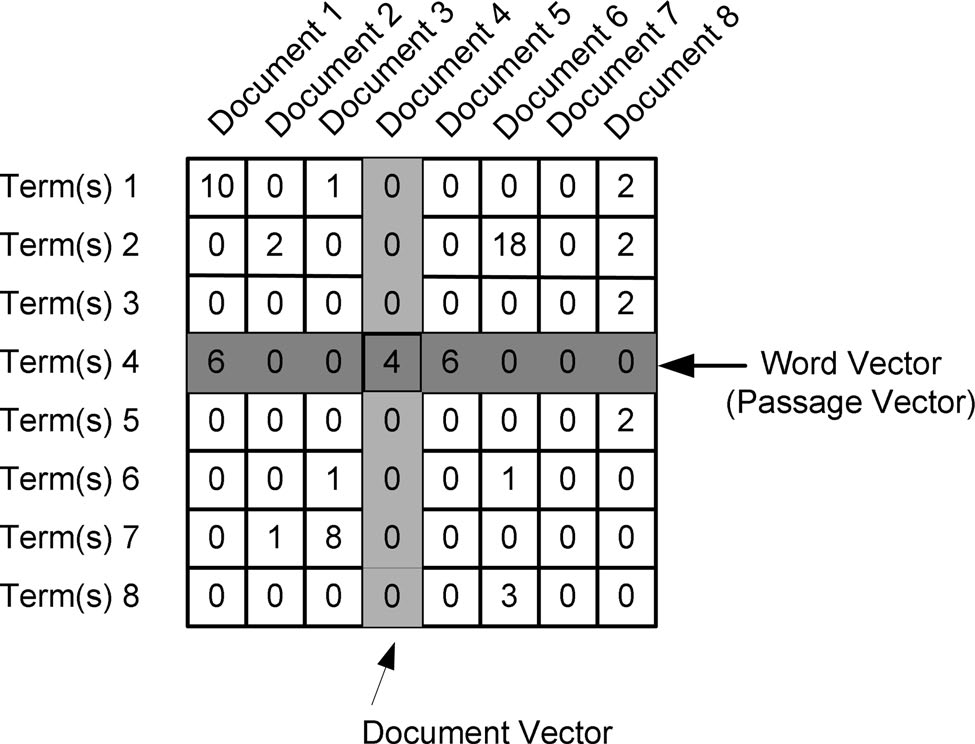
\includegraphics[scale=0.3]{img/VSM}
	\caption{Vektorinės erdvės modelio pavizdys: eilutės žodžių vektoriai, stulpeliai dokumentų vektoriai. \\
	Šaltinis: \cite{marksberry2014employee}}
  \label{vec}
\end{figure}






\subsubsection{Terminų dažnis}

\ltang{Terminų dažnis}{term frequency} (toliau TF) vienas pirmųjų
ir paprasčiausių svėrimo metodų. Tekstų rinkinyje dokumentai, kurie
priklauso tai pačiai temai, labiau tikėtina, kad naudos panašius
žodžius. Taigi, dažniau pasikartojantys žodžiai bus geri tam tikrų temų
indikatoriai.

Yra įvairių būdų apskaičiuoti TF, bet populiariausias – suskaičiuoti
kiek kartų terminas \textit{t} pasikartojo konkrečiame dokumente \textit{d}
(panašiai kaip žodžių maišo metodas).

$$\mathrm{tf} (t,d)=f_{t,d}$$





\subsubsection{Atvirkštinis dokumentų dažnis
(IDF)}

Nors TF yra efektyvus terminų parinkimui, bet jis nėra efektyvus
priskiriant jiems svorius, nes terminai su panašiais svoriais gali
turėti drastiškai skirtingus pasiskirstymus. Žodis, kuris dažnai
pasirodo visuose dokumentuose (pvz., jungtukas „ir“) turės didelę TF
reikšmę, bet visiškai nepadės mums suskirstyti dokumentų į grupes. Tuo
tarpu žodis, pasirodantis mažoje dokumentų grupėje, gali būti kur kas
vertingesnis. Todėl, norėdami sureguliuoti terminų svorius, naudojame
\ltang{atvirkštinį dokumentų dažnį}{inverse document frequency}
(toliau IDF).

IDF išmatuoja ar terminas yra dažnas, ar retas tarp visų dokumentų. Tai
populiariausias ir paprasčiausias metodas ir skaičiuojamas taikant
formulę:

$$\mathrm{idf}(t, D) =  \log \frac{N}{|\{d \in D: t \in d\}|}$$
$N$ – bendras dokumentų kiekis,\\
$|\{d \in D: t \in d\}|$ – kiek dokumentų turi terminą t.\\
Taigi, IDF reikšmė bus didesnė retiems terminams, mažesnė – dažniems ir
lygi 0 terminams, kurie pasitaiko visuose dokumentuose.

IDF pirmą kartą buvo paminėta \cite{sparck1972statistical} ir
paremta empiriniais tyrimais, kurie rodo, kad beveik pusė žodžių yra
sutinkami tekstyne tik po vieną kartą \cite{piaseckiene2014statistiniai}. Šis
reiškinys yra žinomas kaip Zipfo dėsnis.





\subsubsection{TF-IDF}

\ltang{TF-IDF}{term frequency-inverse document frequency} yra
vienas populiariausių žodžių svėrimo metodų {[}Research-paper
recommender systems: a literature survey{]}. Jį gauname sujungus
anksčiau minėtus metodus į vieną\footnote{Dirbant su skirtingos apimties
  dokumentais, yra būdai svoriams normalizuoti atsižvelgiant į dokumentų
  dydį.}:

  $${\displaystyle \mathrm {tfidf} (t,d,D)=\mathrm {tf} (t,d)\cdot \mathrm {idf} (t,D)}$$
TF-IDF apibrėžimo seka kelios savybės:

\begin{itemize}
\item
  Didžiausi svoriai priskiriami terminams, kurie dažnai pasirodo mažoje
  dokumentų grupėje.
\item
  Tarp daugumos dokumentų pasirodantys žodžiai turės mažesnius svorius,
  o žodis aptinkamas visuose dokumentuose svers 0.
\end{itemize}

Šie metodai gali ypač padėti tais atvejais, kai neturime nereikšmingų
žodžių žodyno. Šiame žingsnyje net galime sumažinti žodyno dydį:
panaikindami žodžius, kurie pasikartoja visuose ar daugumoje dokumentų
ir žodžius, kurie pasirodo tik viename dokumente, nes abiem atvejais jie
nebus vertingi klasterizavime.





\subsubsection{Kiti metodai}

Šiame skyriuje aprašyti metodai turėjo keletą rimtų trūkumų, todėl
tokioms problemoms spręsti yra sukurta keletas skirtingų metodų:

\begin{itemize}
\item
  Iš kasdienio gyvenimo žinome, kad vieni žodžiai yra tikėtina dažniau
  sutinkami nei kiti. Todėl pavertus juos vektoriais, negalime tikėtis,
  kad jie bus tiesiškai nepriklausomi. Tokie metodai kaip
  \textbf{word2vec} atsižvelgia į žodžių artumą, kuriant vektorius \cite{mikolov2013efficient}.
\item
  Išskaidydami tekstus į atskirus žodžius, prarandame informaciją apie
  jų eiliškumą. Egzistuoja metodai, kurie atsižvelgia į aplinkinius
  žodžius, kuriant vektorius pvz., \textbf{GloVe} \cite{pennington2014glove}.
\end{itemize}









\section{Klasterizavimo algoritmų analizė}

Klasterizavimas tai viena iš neprižiūrimo mokymosi sričių. Jos tikslas
– sugrupuoti duomenis į klasterius, neturint ankstesnės informacijos
kaip jie turėtų atrodyti.

\begin{itemize}
\item
  \textbf{Atstumas} – Visų pirma, turime apibrėžti atstumo tarp
  analizuojamų objektų (duomenų) matą. Yra sukurta daugybė skirtingų
  matų ir dažnai jų parinkimas priklauso nuo to, kokius duomenis
  analizuojame. Ankstesniuose žingsniuose tekstus pavertėme į
  skaitmeninius duomenis, todėl galime panaudoti daugumą populiarių
  matų.
\end{itemize}

Klasterizavimo metodai:

\begin{itemize}
\item
  \ltang{\textbf{K-vidurkių}}{k-means} – šis metodas sukuria
  \textit{k} centroidų, kurie atitinka klasterio objektų reikšmių vidurkį.
  Tada iteratyviai vis tikslinama, kurie objektai kuriam centroidui
  turėtų priklausyti ir kokioje padėtyje turėtų būti patys centroidai.
  Galiausiai, kai skirstymas stabilizuojasi, turime sudarytus
  klasterius.
\item
  \ltang{\textbf{Lūkesčių-maksimizavimo}}{expectation–maximization} – veikimo principas
  labai panašus į k-vidurkių metodą, tik vietoje centroidų naudojami
  Gauso pasiskirstymai. To rezultate, objektai priklauso kiekvienam
  klasteriui su tikimybe.
\item
  \ltang{\textbf{Hierarchinis}}{hierarchical} – skirtingai nei
  ankstesni metodai, šis sugeneruoja ne atskirus klasterius, bet
  klasterių hierarchiją. Dėl to galime duomenyse atrasti kur kas
  sudėtingesnes struktūras. Bet šis metodas reikalauja, kad papildomai
  apibrėžtume kaip matuojami atstumai tarp klasterių.
\item
  \ltang{\textbf{DBSCAN}}{density-based spatial clustering of
  applications with noise} – metodas kurdamas klasterius remiasi
  objektų tankiu. Objektai, kurie turi šalia savęs pakankamai kaimyninių
  objektų, virsta klasteriais ir plečiasi kol surenka visus pakankamai
  tankius kaimyninius objektus. Šis metodas sėkmingai ignoruoja
  triukšmą, laikydamas jį nepakankamai tankia zona. Taip pat gali
  sudaryti sudėtingos formos klasterius, vienas klasteris gali net
  pilnai apsupti kitą.
\end{itemize}

Be šių yra dar daugybė skirtingų klasterizavimo metodų ir modifikacijų.
Nėra vieno geriausio universalaus metodo, kiekvienas iš jų turi
privalumų ir trūkumų, todėl reikia parinkti metodą, atsižvelgus į
turimus duomenis ir norimus gauti rezultatus.









\section{Kokybės vertinimas}

Visi klasterizavimo metodai turi bendrą silpnybę – jų paskirtis atrasti
duomenų struktūras, tačiau jie gali atrasti jas ir tais atvejais, kai
duomenyse nėra jokių struktūrų {[}Theodoridis; Koutroumbas, 2003{]}.
Todėl klasterizavimo \ltang{kokybės įvertinimas}{evaluation} yra
vienas svarbiausių klasterizavimo proceso etapų. Jo metu gauti
rezultatai parodo ar objektai (duomenys) buvo teisingai sugrupuoti į
klasterius be išankstinės informacjos apie grupes. Egzistuoja 4
kriterijai klasterizavimo rezultatų kokybei įvertinti \cite{feldman2007text}: 

\begin{enumerate}
\item
  \ltang{\textbf{Vidiniai}}{internal} kriterijai kokybę vertina
  lygindami objektų vienoduose klasteriuose panašumą ir objektų skirtumą
  skirtinguose klasteriuose. Deja, šio tipo kriterijai nėra universalūs,
  skirtingiems klasterizavimo metodams reikia parinkti skirtingus
  vidinius kriterijus.
\item
  \ltang{\textbf{Išoriniai}}{external} kriterijai kokybę vertina
  lygindami gautus klasterius su jau iš anksto žinomomis duomenų
  klasėmis. Taigi, šiuo atveju vertiname neprižiūrimo mokymosi metodus
  su prižiūrimo mokymosi problemoms parengtais duomenimis. Nors labai
  tikėtina, kad neprižiūrimo mokymosi metodu sugeneruoti rezultatai bus
  blogesni, bet tai vis tiek labai vertingas vertinimo metodas. Tačiau
  svarbu atkreipti dėmesį, kad duomenis dažnai galima sugrupuoti keliais
  skirtingais būdais ir su duomenimis atėjusios \ltang{etiketės}{labels} nebūtinai yra vienintelis galimas variantas. 
\item
  \ltang{\textbf{Rankiniai}}{manual} kriterijai, kai kokybė yra
  vertinama žmogaus. Praktikoje tokiu būdu visų sudarytų klasterių
  vertinimas užimtų labai daug laiko. Todėl dažniausiai vertintojui
  duodama pora objektų ir klausiama ar jie turėtų būti kartu, ar
  atskirai. Surinkę pakankamai rezultatų iš vertintojų, palyginame su
  rezultatais, gautais taikant klasterizavimo algoritmą. Taip pat šiuo
  atveju galima taikyti duomenų vizualizaciją, deja tai tampa ypač
  sudėtinga su didelės apimties duomenimis (tekstiniais dokumentais).
\item
  \ltang{\textbf{Netiesioginiai}}{indirect} kriterijai įvertina ar
  klasterizavimas yra vertingas žingsnis, didesnės problemos sprendimui
  (pvz., klasterizavimas naudojamas vaizdų atpažinimui kaip tarpinis
  žingsnis matmenų kiekiui sumažinti). Todėl galime stebėti didesnės
  problemos sprendimo rezultatus su skirtingais klasterizavimo metodais
  (ar jų parametrais) ir parinkti tinkamiausią metodą.
\end{enumerate}

Praktikoje, jei yra galimybė, dažniausiai naudojami išoriniai
kriterijai, keletas jų yra:

\begin{enumerate}
\item
  \textbf{Rand indeksas} (toliau Rand) \cite{rand1971objective} – teisingai suklasterizuotų
  objektų dalis:

  $$Rand={\frac {TP+TN}{TP+FP+FN+TN}}$$

  \begin{table}[h]
  \caption{Klasterių kokybės vertinimas}
	\begin{tabular}{|c|c|c|}
	\hline
							& Priklauso klasei                                                                              & Nepriklauso klasei                                                                          \\ \hline
	Priskirtas klasteriui   & \begin{tabular}[c]{@{}c@{}}Teisingai priskirtas\\ (angl. \textit{true positive})\\(TP)\end{tabular}      & \begin{tabular}[c]{@{}c@{}}Neteisingai priskirtas\\ (angl. \textit{false positive})\\(FP)\end{tabular} \\ \hline
	Nepriskirtas klasteriui & \begin{tabular}[c]{@{}c@{}}Neteisingai nepriskirtas\\ (angl. \textit{false negative})\\(FN)\end{tabular} & \begin{tabular}[c]{@{}c@{}}Teisingai nepriskirtas\\ (angl. \textit{true negative})\\(TN)\end{tabular}  \\ \hline
  \end{tabular}
  \label{truefalse}
  \end{table}

\item
  \ltang{Homogeniškumas}{homogeneity} \cite{rosenberg2007v} –
  kiekvienam klasteriui priklauso objektai tik iš vienos klasės:

  $$h={1-\frac {H(C|K)}{H(C)}}$$
  $$H(C)=-\sum_{c=1}^{|C|}{\frac {n_c}{n}\cdot\log \left(\frac {n_c}{n}\right)}$$
  $$H(C|K)=-\sum_{c=1}^{|C|}\sum_{k=1}^{|K|}\frac{n_{c,k}}{n}\cdot\log\left(\frac{n_{c,k}}{n_{k}}\right)$$

\item
  \ltang{Išsamumas}{completeness} \cite{rosenberg2007v} visi
  klasės objektai priklauso tik vienam klasteriui.

  $$c={1-\frac {H(K|C)}{H(K)}}$$
\end{enumerate}










\section{Eksperimentinis tyrimas}

Dokumentų klasterizavimo eksperimentiniam tyrimui duomenų šaltiniu
pasirinkau naujienų svetainės „Delfi“ 5 skirtingų kategorijų 2017 m.
paskelbtus straipsnius ir, taikydamas skirtingus klasterizavimo metodus,
bandžiau šiuos straipsnius priskirti pasirinktoms svetainės
kategorijoms.

Eksperimento metu išbandžiau keturis kursiniame darbe paminėtus
klasterizavimo algoritmus, o duomenis parengiau šiame darbe paminėtais
būdais ir įvertinau gautų klasterių kokybę.






\subsection{Duomenų išgavimo rezultatai}

Pirmas eksperimentinio tyrimo žingsnis buvo gauti naujienų straipsnius.
Neradęs jau paruošto duomenų rinkinio ar patogios
sąsajos atsisiųsti didelius kiekius straipsnių iš populiariausių
naujienų svetainių (\url{https://www.delfi.lt/},
\url{https://www.lrytas.lt/}, \url{https://www.15min.lt/},
\url{https://www.alfa.lt/}, \url{https://www.tv3.lt/}), su prašymu dėl
tokios galimybės suteikimo kreipiausi į šias agentūras elektroniniu
paštu. Tačiau naujienų agentūroms neatsiliepus į mano prašymą, ir, kad
galėčiau tyrimo metu pasinaudoti naujienų svetainių straipsniais,
nusprendžiau parašyti savo internetinį robotą. Internetiniam robotui rašyti pasinaudojau Scrapy
biblioteka\footnote{\url{https://scrapy.org/}} (Programos kodas \ref{code} priede).

Iš anksčiau išvardintų lietuviškų naujienų svetainių darbui pasirinkau
„Delfi“. Tokį pasirinkimą lėmė šios svetainės plati straipsnių
įvairovė, straipsnių puslapiuose esanti papildoma vertinga
informacija\footnote{Ne tik pavadinimas ir tekstas, bet ir parašymo
  data, kategorija, \ltang{įvadas}{intro} ir \ltang{žymės}{tags}} ir svarbiausia, archyvo funkcija\footnote{https://www.delfi.lt/archive/},
kur galima atlikti straipsnių paiešką pagal raktinį žodį, datą ir
kategoriją. Nusprendžiau išgauti 2017 m. sausio 1 d.–gruodžio 31 d.
archyve iš 5-ių skirtingų kategorijų po 1000 straipsnių. Kategorijas
pasirinkau remdamasis tuo, kad, mano manymu, jas galėtų lengvai atskirti
vieną nuo kitos eilinis vartotojas. Pasirinktos šios kategorijos:
„Auto“, „Veidai“, „Sportas“, „Mokslas“ ir „Verslas“.

Po to, internetinio roboto pagalba išgavęs reikiamus straipsnius
(duomenų rinkinį), atlikau duomenų valymą: panaikinau blogai nuskaitytus
straipsnius (keletas straipsnių turėjo išskirtinį formatavimą nors
vizualiai atrodė identiškai) ir straipsnius, turinčius mažiau nei 1000
simbolių tekstą (iš 5233 nuskaitytų straipsnių tolesnei analizei liko
4058\footnote{Auto – 895, Veidai – 779, Sportas – 760, Mokslas –
  837, Verslas – 787 straipsnių; vidutiniškai 812 straipsnių.}, arba 78
\% straipsnių). Tada, kad galėčiau straipsnius priskirti atitinkamoms
kategorijoms, suvienodinau jų pavadinimus (pvz., „Auto“, „auto“,
„Delfi auto“ pakeičiau į „Auto“).






\subsection{Teksto filtravimo ir požymių išskyrimo rezultatai}

Teksto filtravimui atlikau leksinę analizę, nereikšmingų žodžių
panaikinimą ir kamieno atskyrimą. Sinonimų ir daugiareikšmių žodžių
analizatoriaus ir lemuoklio, kuriuos galėčiau panaudoti dideliems
kiekiams lietuviškų tekstų, nepavyko rasti\footnote{VDU suteikia prieiga
  prie internetinio morfologinio anotatoriaus
  \url{http://donelaitis.vdu.lt/main.php?id=4\&nr=7_2}, bet nėra
  patogaus būdo atlikti analizę su dideliais tekstų kiekiais.}.

Leksinei analizei panaudojau \ltang{reguliarųjį reiškinį}{regular
expression}: „\texttt{{[}\textbackslash{}W\textbackslash{}d\_{]}+}“, kad
pakeisčiau visus simbolius, kurie nėra raidės (\texttt{\textbackslash{}W})
ir skaičius (\texttt{\textbackslash{}d}) į tarpo simbolį ir tada tekstą
suskaldžiau pagal tarpo simbolius. Nors yra keli atvejai, kai šis
metodas neidealiai susitvarko su tekstu ( „1992-ųjų“, romėniškais
skaičiais, „2 mln.“), bet manau gauti rezultatai yra pakankamai geri.
Straipsnius sudarė vidutiniškai 415 žodžių ( trumpiausias – 97, o
ilgiausias – 3335 žodžius).

Nereikšmingiems žodžiams pašalinti pasinaudojau jau sudarytu
žodynu\footnote{\url{https://gist.github.com/revelt/01524e76c6e5e0970d2d0fe8797e92ed}}(Pilnas
žodynas \ref{stopWords} priede). Iš kiekvieno straipsnio pašalinta vidutiniškai po 85
žodžius arba \textasciitilde{}21\% žodžių.

Kamieno atskyrimui nusprendžiau panaudoti populiarią, taisyklėmis
paremtą sistemą „Snowball“. Ši sistema atlieka analizę pagal pateiktas
taisykles, todėl kiekvienai kalbai jos turi būti realizuotos atskirai.
Populiariausia šios sistemos realizacija\footnote{\url{https://snowballstem.org/}}
yra ir lietuvių kalba\footnote{\url{https://github.com/snowballstem/snowball/blob/master/algorithms/lithuanian.sbl}}.
Duomenų rinkinyje iš viso buvo 141370 unikalūs žodžiai, išgavus
kamienus, liko 47707 unikalūs žodžių kamienai.

Požymių išskyrimui naudojau Scikit-learn\footnote{\href{https://scikit-learn.org/stable/modules/clustering.html}{https://scikit-learn.org}}
bibliotekoje realizuotą tf-idf metodą. Be papildomų nustatymų šis
metodas grąžino 4058×47581 dydžio matricą (4058 – atskiri dokumentai,
47581 – požymiai). Deja, ši matrica buvo per didelė porai metodų (LM ir
hierarchinio jungiamojo), todėl nusprendžiau pasinaudoti
„\textit{max\_features}“ parametru ir palikti pusę požymių (23790).
K-vidurkių ir DBSCAN metodai nebuvo smarkiai to paveikti.






\subsection{Klasterizavimo metodai ir jų parametrų parinkimas}

Klasterizavimui taip pat naudojau Scikit-learn biblioteką. Ši biblioteka
realizuoja daug skirtingų klasterizavimo metodų\footnote{\url{https://scikit-learn.org/stable/modules/clustering.html}},
įskaitant ir mano analizuotus: K-vidurkių, lūkesčių-maksimizavimo,
hierarchinio jungiamojo ir DBSCAN. Kiekvienas iš metodų turi papildomus
parametrus, kuriuos galima nustatyti prieš klasterizavimą. Keletas
prasmingų ir susijusių su mano ankstesne apžvalga parametrų:

\begin{itemize}
\item
  K-vidurkių

  \begin{itemize}
    \item
    \texttt{n\_clusters} – šis parametras nurodo, kiek klasterių bus
    sudaryta ir tuo pačiu kiek centroidų, kitaip tariant, tai atitinka
    \textit{k}. Kadangi straipsnius parinkau iš 5 kategorijų, todėl šį
    parametrą taip pat nustačiau 5.
  \item
    \texttt{init} – centroidų inicijavimo metodas. Pasirinkau
    k-means++.
  \item
    \texttt{n\_init} – ši k-vidurkių realizacija lokalaus maksimumo
    problemą sprendžia pakartotinai paleidžiant metodą ir šis parametras
    nurodo kiek kartų tai bus atlikta. Šiuo atveju palikau numatytą
    reikšmę – 10.
  \item
    \texttt{max\_iter} – kiek iteracijų atlikti, palikau numatytą
    reikšmę – 300.
  \item
    \texttt{random\_state} – k-vidurkių veikimui reikalingos
    atsitiktinės reikšmės, todėl norint rezultatus padaryti
    deterministinius, galima nurodyti \ltang{atsitiktinumo inicializavimo
    reikšmę}{random seed}. Kad rezultatai tarp skirtingų
    bandymų išliktų stabilūs ir nepriklausytų nuo atsitiktinumo,
    nustačiau inicializavimo reikšmę – 42.
  \end{itemize}
\item
  Lūkesčių-maksimizavimo

  \begin{itemize}
    \item
    \texttt{n\_components} – atitinka k-vidurkių parametrą
    \texttt{n\_clusters}.
  \item
    \texttt{n\_init, max\_iter, random\_state}
    – reiškia tą patį kaip ir k-vidurkių parametrai. \texttt{n\_init,
    max\_iter} palikau numatytas reikšmes, atitinkamai 1 ir
    100, \texttt{random\_state} nustačiau 42.
  \item
    \texttt{init\_params} – inicializavimo metodas. Čia palikau
    „k-means“ numatytą reikšmę.
  \end{itemize}
\item
  Hierarchinio jungiamojo

  \begin{itemize}
    \item
    \texttt{n\_clusters} – atitinka k-vidurkių parametrą.
  \item
  	\texttt{Linkage} –
    nurodo atstumo matavimo /
    jungimo metodą. Palaikomieji: tolimiausio
    kaimyno, vidutinių atstumų ir Ward
    metodas. Išbandžiau visus atskirai.
  \end{itemize}
\item
  DBSCAN

  \begin{itemize}
    \item
    \texttt{eps, min\_samples} –
    maksimalus atstumas iki kaimyno ir
    minimalus kaimynų
    kiekis. Kaip parinkau šiuos parametrus aprašyta
    prie rezultatų(\ref{dbscanRes}).
  \end{itemize}
\end{itemize}

Skirtingų metodų implementacijos skirtingai palaiko panašumo
funkcijas / įverčius, todėl nusprendžiau palikti numatytas reikšmes.





\subsection{Rezultatai ir jų vertinimas}

Kadangi iš anksto buvo žinomos straipsnių kategorijos (kurias galime
laikyti klasėmis), todėl rezultatų vertinimui naudojau išorinius
kriterijus. Tuo tarpu lyginant skirtingų klasterizavimo metodų
rezultatus, vidiniai kriterijai nėra tinkami, nesvieni iš jų būtų palankesni vieniems metodams, kiti kitiems.

Žinant šias sąlygas nusprendžiau klasterizavimo rezultatus vertinti 4
skirtingais būdais\footnote{1 ir 2 galime laikyti rankiniu vertinimu, o
  3 ir 4 išoriniu.}:

\begin{enumerate}
\item
  Pagal tinkamiausius požymius – k-vidurkių ir lūkesčių-maksimizavimo
  metodų sudaryti klasteriai turi centrus, todėl galime nustatyti, kurie
  požymiai geriausiai juos atitinka. Kiekvieno klasterio 10 tinkamiausių
  požymių pateikiau lentelėse.
\item
  Stebint klasterių dydžius – kiekvienai kategorijai priklauso panašus
  kiekis duomenų, todėl vien tik stebint sudarytų klasterių dydžius,
  galima spręsti apie jų kokybę.
\item
  Pagal išorinius kriterijus – Scikit-learn biblioteka palaiko daug
  klasterių vertinimo metodų ir visus iš mano paminėtų: Rand
  indeksas(Rand), homogeniškumas ir išsamumas.
\item
  Naudojant \ltang{sumišimo matricą}{confusion matrix} –
  pavaizduojama kiek straipsnių yra kategorijose ir į kurį klasterį jie
  pateko\footnote{\ref{truefalse} lentelę galima laikyti 2 klasterių sumišimo matrica}.
  Idealiu atveju (Stulpelių eilės tvarka nesvarbi), matrica atrodytų taip:
  \begin{figure}[H]
	\centering
	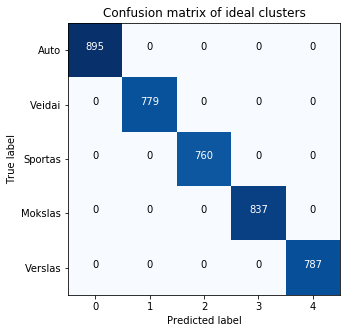
\includegraphics[width=2.7953in,height=2.5984in]{./Pictures/100002010000015E0000014D6F097C7C354B2FCC.png}
	\caption{Ideali Sumišimo matrica}
  \end{figure}
\end{enumerate}

2, 3 ir 4 vertinimus pateikiu dvejomis formomis. Pirma – tokius, kaip
jie atrodė iš karto po klasterizavimo, kai jų eiliškumas buvo
atsitiktinis ir antra – perrikiavus, kad būtų lengviau pastebėti, kurią
kategoriją jie geriausiai atitinka. Šis perrikiavimas veikia taip:
kiekvienam klasteriui priskiriame naują indeksą pagal tai, kuriai
kategorijai daugiausia jo elementų priklauso. To pasekoje, klasteriai
gali būti sujungti į vieną (tai ypač svarbu, jei klasterių skaičius būtų
didesnis nei kategorijų).





\subsubsection{K-vidurkių rezultatai}

\begin{table}[!h]
	\footnotesize
	\caption{Tinkamiausi klasterių požymiai}

	\begin{tabular}{|c|l|l|l|l|l|l|l|l|l|l|}
	\hline
	Klasteris & \multicolumn{10}{c|}{Požymiai} \\ \hline
	0 & rungtyn & komand & įvart & žaid & lyg & tašk & klub & ekip & pergal
	& rinktin\\ \hline
	1 & yr & buv & met & kur & film & žmon & lab & gal & dain &
	vis\\ \hline
	2 & eur & proc & met & lietuv & darb & yr & įmon & kain & telefon &
	kur\\ \hline
	3 & automobil & vair & eism & transport & model & kel & priemon & varikl
	& gal & yr\\ \hline
	4 & sport & varžyb & sportinink & lietuv & lenktyn & ral & met & čempion
	& viet & olimpin\\ \hline
	\end{tabular}
\end{table}

\begin{table}[!h]

\begin{tabular}{ll}

	\begin{minipage}[t]{0.47\columnwidth}\raggedright
		Klasterių dydžiai: {[} 393 1322 1221 671 451{]}\\
		Rand: 0.450\\
		Homogeniškumas: 0.535\\
		Išsamumas: 0.576

		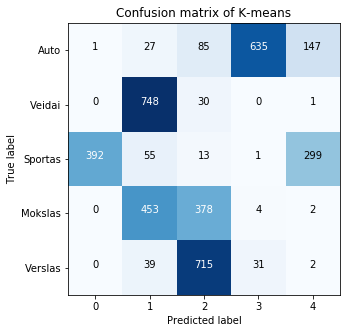
\includegraphics[width=\columnwidth]{./Pictures/100002010000015E0000014D2A34E945EE2F9B27.png}\strut
		\center{a)}
	\end{minipage}
	&
	\begin{minipage}[t]{0.47\columnwidth}\raggedright
		Klasterių dydžiai: {[} 671 1322 844 0 1221{]}\\
		Rand: 0.489\\
		Homogeniškumas: 0.519\\
		Išsamumas: 0.618		

		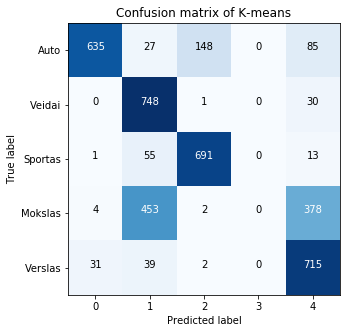
\includegraphics[width=\columnwidth]{./Pictures/100002010000015E0000014D77AD2EBC2026345C.png}\strut
		\center{b)}
	\end{minipage}
\end{tabular}
\captionof{figure}{K-vidurkių algoritmo rezultatų sumišimo matrica a) nerikiuota ; b) rikiuota}
\end{table}

Kaip matyti iš sumišimo matricos, k-vidurkių metodu visų kategorijų
straipsniai buvo suskirstyti gana teisingai, išskyrus „Sporto“ ir
„Mokslo“ kategorijų straipsnius. „Sporto“ kategorijos straipsniai
pasidalino į du klasterius (0 ir 4), „Mokslo“ straipsniai irgi
pasidalino į du klasterius (1 ir 2), be to, dar susimaišė su kitomis
kategorijomis („Veidai“ ir „Verslas“). „Auto“ kategorijos straipsniai
buvo sėkmingai atskirti.

Tai ką matome tarp straipsnių pasiskirstymo, taip pat galime pastebėti
ir tinkamiausių požymių lentelėje. Vien tik skaitant juos, galime
nuspėti kategorijų pavadinimus. Vienintelė išimtis 1 klasteris, pagal
kurio požymius ( pvz.: „yr“, „buv“, „met“\ldots{}) sunkiau nuspėti
temą, kuriai būtų galima priskirti.

Perrikiavus duomenis, 0 ir 4 klasteriai susijungė į vieną, „Sporto“
kategoriją reprezentuojantį klasterį.





\subsubsection{Lūkesčių-maksimizavimo (LM)
rezultatai}

\begin{table}[!h]
	\footnotesize
	\caption{Tinkamiausi klasterių požymiai}

	\begin{tabular}{|c|l|l|l|l|l|l|l|l|l|l|}
	\hline
	Klasteris & \multicolumn{10}{c|}{Požymiai} \\ \hline
	0 & mokslinink & yr & tyrim & žem & gal & kur & kosm & planet & met &
	buv\\ \hline
	1 & film & buv & yr & kur & met & dain & lab & koncert & vis &
	telefon\\ \hline
	2 & eur & proc & met & darb & lietuv & įmon & yr & kain & mokest &
	mln\\ \hline
	3 & komand & rungtyn & lietuv & čempion & įvart & tašk & pergal & viet &
	varžyb & žaid\\ \hline
	4 & automobil & vair & eism & transport & model & kel & gal & priemon &
	varikl & yr\\ \hline
	\end{tabular}
\end{table}

\begin{table}[!h]
\begin{tabular}{ll}
	\begin{minipage}[t]{0.47\columnwidth}\raggedright
		Klasterių dydžiai: [386 1144 1035  785  708]\\
		Rand: 0.545\\
		Homogeniškumas: 0.583\\
		Išsamumas: 0.604

		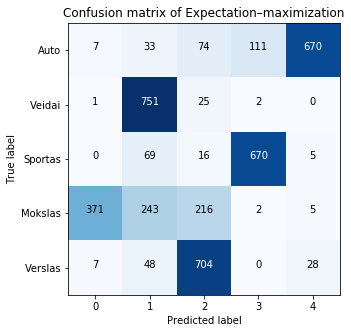
\includegraphics[width=\columnwidth]{./Pictures/100002010000015F0000014DCC9137F85916128D.png}\strut
		\center{a)}
	\end{minipage}
	&
	\begin{minipage}[t]{0.47\columnwidth}\raggedright
		Klasterių dydžiai: [708 1144  785  386 1035]\\
		Rand: 0.545\\
		Homogeniškumas: 0.583\\
		Išsamumas: 0.604
		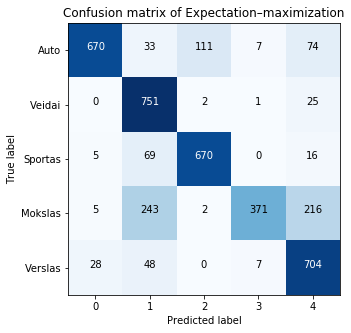
\includegraphics[width=\columnwidth]{./Pictures/100002010000015F0000014D3D8F881D4BB6DB07.png}\strut
		\center{b)}
	\end{minipage}
\end{tabular}
\captionof{figure}{Lūkesčių-maksimizavimo algoritmo rezultatų sumišimo matrica a) nerikiuota ; b) rikiuota}
\end{table}

LM metodas, kaip buvo galima tikėtis, sugeneravo į k-vidurkių metodą
labai panašius klasterius. „Mokslas“ straipsniai pasiskirstė tarp trijų
klasterių, du („Veidai“ ir „Verslas“) susimaišė su kitų kategorijų
straipsniais ir vienas klasteris liko atskiras nuo kitų. „Auto“ ir
„Sporto“ straipsniai buvo sėkmingai suklasterizuoti į atskirus
klasterius.

Pagal klasterių požymius lengvai galime išskirti 5-ias kategorijas. Taip
pat pagal šiuos rezultatus galima lengviau (nei k-vidurkių atveju)
pastebėti apie ką rašo „Veidas“ kategorijos straipsniai. Išsiskiria
požymiai: „film“, „dain“, „koncert“ – aiškiai kalbama apie
pramoginius renginius.

Po perrikiavimo jokie klasteriai nesusijungė, tik pasikeitė jų
eiliškumas.





\subsubsection{Hierarchinio jungiamojo rezultatai}

\textbf{Tolimiausio kaimyno}

\begin{table}[!h]
	\begin{tabular}{ll}
	
		\begin{minipage}[t]{0.47\columnwidth}\raggedright
			Klasterių dydžiai: [2096 1079 229 519 135]\\
			Rand: 0.169\\
			Homogeniškumas: 0.255\\
			Išsamumas: 0.332
	
			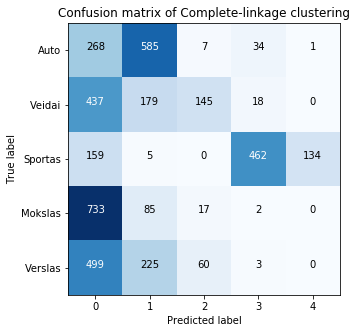
\includegraphics[width=\columnwidth]{./Pictures/10000201000001650000014DB994A3E776C8BF67.png}\strut
			\center{a)}
		\end{minipage}
		&
		\begin{minipage}[t]{0.47\columnwidth}\raggedright
			Klasterių dydžiai: [1079 229 654 2096 0]\\
			Rand: 0.195\\
			Homogeniškumas: 0.253\\
			Išsamumas: 0.354
			
			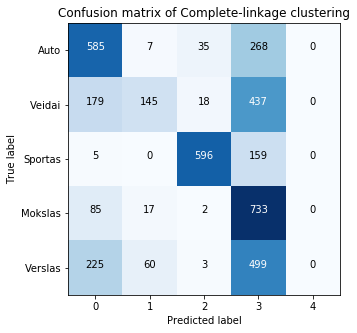
\includegraphics[width=\columnwidth]{./Pictures/10000201000001650000014D320329FEFC52B260.png}\strut
			\center{b)}
		\end{minipage}
	\end{tabular}
	\captionof{figure}{Tolimiausio kaimyno metodo rezultatų sumišimo matrica a) nerikiuota ; b) rikiuota}
\end{table}

Iš pateiktų sumišimo martricų matome, kad tolimiausio kaimyno metodo
pateikti rezultatai buvo prasti. Į 0 klasterį pateko daugiau nei pusė
visų straipsnių. Sėkmingai į du atskirus klasterius buvo atskirti tik
„Sportas“ kategorijos straipsniai. Kiti klasteriai buvo sudaryti iš
kelių kategorijų. Perrikiavus, du „Sporto“ klasteriai susijungė į
vieną.

\textbf{Vidutinių atstumų}

\begin{table}[!h]
	\begin{tabular}{ll}
	
		\begin{minipage}[t]{0.47\columnwidth}\raggedright
			Klasterių dydžiai: [4049 3 2 1 3]\\
			Rand: 0.000\\
			Homogeniškumas: 0.002\\
			Išsamumas: 0.165\\
			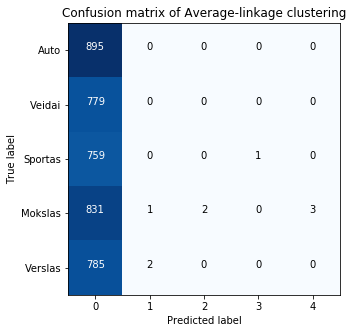
\includegraphics[width=2.9465in,height=2.7799in]{./Pictures/10000201000001610000014D78BBE2D1F67B03F8.png}
			\captionof{figure}{Vidutinių atstumų metodo rezultatų sumišimo matrica}
		\end{minipage}
		&
		\begin{minipage}[t]{0.47\columnwidth}\raggedright
			Kaip parodė tyrimo rezultatai, mažiausiai tinkamas lietuviškų tekstų
			klasterizavimui buvo vidutinių atstumų metodas. Pritaikius šį metodą,
			praktiškai visi straipsniai buvo priskirti vienam klasteriui.
		\end{minipage}
	\end{tabular}
	\end{table}


\textbf{Ward metodas}

\begin{table}[!h]
	\begin{tabular}{ll}
	
		\begin{minipage}[t]{0.47\columnwidth}\raggedright
			Klasterių dydžiai: [1828 502 680 404 644]\\
			Rand: 0.385\\
			Homogeniškumas: 0.488\\
			Išsamumas: 0.545
	
			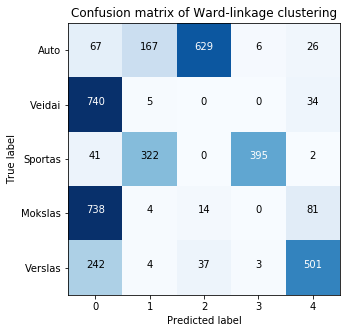
\includegraphics[width=\columnwidth]{./Pictures/100002010000015E0000014D462E1B8414920DD7.png}\strut
			\center{a)}
		\end{minipage}
		&
		\begin{minipage}[t]{0.47\columnwidth}\raggedright
			Klasterių dydžiai: [680 1828 906 0 644]\\
			Rand: 0.425\\
			Homogeniškumas: 0.473\\
			Išsamumas: 0.591
	
			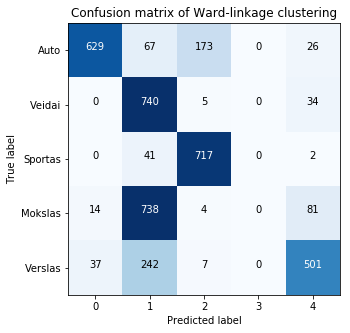
\includegraphics[width=\columnwidth]{./Pictures/100002010000015E0000014DF0AC1DC116DCE84C.png}\strut
			\center{b)}
		\end{minipage}
	\end{tabular}
	\captionof{figure}{Ward metodo rezultatų sumišimo matrica a) nerikiuota ; b) rikiuota}
\end{table}

Klasterizuojant lietuviškus dokumentus Ward metodas, manyčiau, kad
galėtų būti taikomas, nes beveik pusė straipsnių buvo priskirti vienam
klasteriui, kiti buvo neblogai atskirti pagal kategorijas. „Auto“ ir
„Verslas“ kategorijos buvo atskirtos į atskirus klasterius, „Sportas“
kategorijos straipsniai padalinti tarp 2 klasterių, o „Veidai“ ir
„Mokslas“ kategorijų straipsniai pateko į vieną klasterį. Perrikiavus,
„Sportas“ kategorijai atitikę klasteriai, susijungė į vieną.






\subsubsection{DBSCAN rezultatai}\label{dbscanRes}

Su DBSCAN metodu buvo sudėtingiau, nes kaip parametro nebuvo įmanoma
nurodyti norimo klasterių skaičiaus, reikėjo išbandyti daug parametrų
reikšmių kombinacijų. Deja, bet nei viena kombinacija nedavė tinkamo
rezultato, todėl pakako stebėti klasterių dydžius ir kiti vertinimo
metodai nebuvo reikalingi. \texttt{eps} parametrui –
išbandžiau reikšmes nuo 0,6 iki 1,3;
\texttt{min\_samples} parametrui – išbandžiau
reikšmes nuo 3 iki 8. Pilna rezultatų lentelė \ref{dbscanTable}
priede. Taikant DBSCAN
metodą gauti tokie pastebėjimai:

\begin{itemize}
\item
  Kai \texttt{eps} reikšmė
  buvo mažesnė nei 0,6, visi duomenys buvo
  priskiriami triukšmui, kai
  reikšmė didesnė nei 1,3 – visi duomenys
  buvo priskiriami vienam klasteriui;
\item
  Didinat \texttt{min\_samples} reikšmę,
  klasterių kiekis ir dydžiai mažėja. Reikšmės
  mažesnės nei 3 buvo netinkamos\footnote{Išsamiau
    apie tai pirmame darbe.};
\item
  Kai \texttt{eps} reikšmės
  buvo nuo 0,6 iki 1,1 (imtinai)
  dauguma duomenų buvo priskiriami
  triukšmui, bet nuo 1,2 ir daugiau –
  dauguma duomenų buvo priskiriami
  vienam klasteriui;
\item
  Dažniausiai sudaromi dideli kiekiai mažų klasterių
  (daugiausia buvo sudaryti 177).
\end{itemize}

Galima daryti išvadą , kad duomenys
buvo per daug tolygaus (nėra atskirų
duomenų „sutirštėjimų“\footnote{Tai
  gali būti dėl didelio duomenų dimensingumo}. 
(anlg. blob) tankio, kad būtų sėkmingai
suklasterizuoti taikant šį
metodą.











\subsection{Išvados}

Eksperimentinio tyrimo metu buvo pasiektas užsibrėžtas tikslas –
aprašyti lietuviškų tekstinių dokumentų parengimo klasterizavimui
žingsniai, palygintas skirtingų klasterizavimo metodų veikimas taikant
juos darbui su lietuviškais dokumentais, įvertinta rezultatų kokybė ir
pateikti pasiūlymai.

1. Tyrimui buvo sudarytas didelės apimties tekstinis duomenų rinkinys iš
5-ių skirtingų kategorijų ir kiekviena kategorija iš vidutiniškai 812
skirtingų straipsnių.

2. Duomenų rinkiniui buvo atlikta leksinė analizė, pašalinti
nereikšmingi žodžiai ir išskirti žodžių kamienai. Tada duomenys buvo
paversti į verktorinę formą naudojant tf-idf metodą.

3. Eksperimentas buvo atliekamas su 4-ių tipų klasterizavimo metodais:
k-vidurkių, lūkesčių-maksimizavimo, hierarchinio jungiamojo
(su tolimiausio kaimyno,
vidutinių atstumų ir Ward
atstumo matavimo / jungimo metodais) ir
DBSCAN.

4. Eksperimento metu gautų rezultatų kokybės vertinimas buvo atliktas
4-iais būdais: tinkamiausių požymių išskyrimo, klasterių dydžių
stebėjimo, taikant išorinius kriterijus ( Rand indeksas, homogeniškumas,
išsamumas) ir sumišimo matricas.

Kaip parodė eksperimentinio tyrimo rezultatai, lietuviškų tekstų
klasterizavimui mažiausiai pritaikytas yra DBSCAN metodas, nes tyrimo
metu buvo gauti prasčiausi rezultatai ir reikalavo daugiausia parametrų
derinimo. Taip pat prasti rezultatai gauti naudojant vidutinių atstumų
ir tolimiausio kaimyno metodus. Ward metodas pateikė pakankamai gerus
rezultatus ir gali būti naudojamas lietuviškų tekstų klasterizavimui.

Dėl rezultatų interpretavimo paprastumo ir geros jų kokybės, skaldantys
/ centroidais paremti metodai geriausiai tinka lietuviškiems tekstiniams
duomenims klasterizuoti. K-vidurkių ir LM metodus galima laikyti
geriausiai pritaikytais lietuviškų tekstų klasterizavimui. K-vidurkių
algoritmo sugeneruoti klasteriai atitiko keturias, o LM algoritmo –
visas penkias kategorijas.

Manau, kad eksperimentinius tyrimus su skirtingai paruoštais
lietuviškais tekstiniais dokumentais ir pritaikant įvairius
klasterizavimo metodus, reikėtų tęsti ir ateityje.











\printbibliography[heading=bibintoc]

\appendix

\section{DBSCAN rezltatų lentelė}\label{dbscanTable}
\begin{table}[!ht]
\footnotesize
\begin{tabular}{|l|l|l|l|l|}
\hline
\textbf{ε} & \textbf{Min} & \textbf{Triukšmas} & \textbf{Klasterių kiekis} & \textbf{10 didžiausių klaserių}           \\ \hline
\rowcolor[HTML]{EFEFEF} 
0.6        & 3            & 3989               & 18                        & 11, 5, 5, 4, 4, 4, 3, 3, 3, 3             \\ \hline
\rowcolor[HTML]{EFEFEF} 
0.6        & 4            & 4025               & 6                         & 11, 5, 5, 4, 4, 4                         \\ \hline
\rowcolor[HTML]{EFEFEF} 
0.6        & 5            & 4037               & 3                         & 11, 5, 5                                  \\ \hline
\rowcolor[HTML]{EFEFEF} 
0.6        & 6            & 4048               & 1                         & 10                                        \\ \hline
\rowcolor[HTML]{EFEFEF} 
0.6        & 7            & 4048               & 1                         & 10                                        \\ \hline
\rowcolor[HTML]{EFEFEF} 
0.6        & 8            & 4048               & 1                         & 10                                        \\ \hline
0.7        & 3            & 3946               & 27                        & 14, 9, 6, 6, 5, 5, 5, 4, 4, 3             \\ \hline
0.7        & 4            & 4001               & 9                         & 14, 9, 6, 6, 5, 5, 4, 4, 4                \\ \hline
0.7        & 5            & 4014               & 6                         & 14, 9, 6, 5, 5, 5                         \\ \hline
0.7        & 6            & 4031               & 3                         & 14, 7, 6                                  \\ \hline
0.7        & 7            & 4037               & 2                         & 14, 7                                     \\ \hline
0.7        & 8            & 4044               & 1                         & 14                                        \\ \hline
\rowcolor[HTML]{EFEFEF} 
0.8        & 3            & 3870               & 47                        & 14, 10, 9, 8, 6, 6, 5, 5, 5, 5            \\ \hline
\rowcolor[HTML]{EFEFEF} 
0.8        & 4            & 3976               & 13                        & 14, 9, 9, 8, 6, 6, 5, 5, 4, 4             \\ \hline
\rowcolor[HTML]{EFEFEF} 
0.8        & 5            & 4001               & 7                         & 14, 9, 9, 8, 6, 6, 5                      \\ \hline
\rowcolor[HTML]{EFEFEF} 
0.8        & 6            & 4012               & 5                         & 14, 9, 9, 8, 6                            \\ \hline
\rowcolor[HTML]{EFEFEF} 
0.8        & 7            & 4018               & 4                         & 14, 9, 9, 8                               \\ \hline
\rowcolor[HTML]{EFEFEF} 
0.8        & 8            & 4027               & 3                         & 14, 9, 8                                  \\ \hline
0.9        & 3            & 3649               & 85                        & 24, 21, 15, 13, 10, 10, 10, 9, 8, 7       \\ \hline
0.9        & 4            & 3801               & 38                        & 23, 21, 15, 12, 10, 10, 10, 9, 7, 7       \\ \hline
0.9        & 5            & 3886               & 19                        & 23, 21, 12, 10, 10, 10, 9, 9, 7, 7        \\ \hline
0.9        & 6            & 3911               & 16                        & 23, 21, 10, 9, 9, 9, 8, 7, 7, 7           \\ \hline
0.9        & 7            & 3950               & 10                        & 23, 21, 10, 9, 9, 8, 7, 7, 7, 7           \\ \hline
0.9        & 8            & 3989               & 5                         & 23, 18, 10, 9, 9                          \\ \hline
\rowcolor[HTML]{EFEFEF} 
1          & 3            & 3172               & 155                       & 39, 33, 33, 27, 23, 19, 17, 16, 13, 12    \\ \hline
\rowcolor[HTML]{EFEFEF} 
1          & 4            & 3428               & 80                        & 39, 33, 30, 27, 23, 19, 15, 13, 13, 12    \\ \hline
\rowcolor[HTML]{EFEFEF} 
1          & 5            & 3566               & 50                        & 39, 33, 27, 25, 23, 19, 13, 13, 12, 12    \\ \hline
\rowcolor[HTML]{EFEFEF} 
1          & 6            & 3654               & 39                        & 33, 28, 27, 23, 22, 19, 13, 12, 12, 12    \\ \hline
\rowcolor[HTML]{EFEFEF} 
1          & 7            & 3778               & 20                        & 31, 28, 25, 23, 22, 19, 12, 12, 12, 11    \\ \hline
\rowcolor[HTML]{EFEFEF} 
1          & 8            & 3831               & 15                        & 31, 28, 23, 20, 19, 17, 12, 12, 10, 10    \\ \hline
1.1        & 3            & 2287               & 177                       & 144, 138, 121, 89, 88, 66, 63, 49, 49, 41 \\ \hline
1.1        & 4            & 2564               & 110                       & 143, 107, 89, 87, 64, 48, 48, 47, 41, 38  \\ \hline
1.1        & 5            & 2763               & 90                        & 131, 75, 70, 60, 48, 41, 41, 38, 37, 36   \\ \hline
1.1        & 6            & 2930               & 71                        & 128, 72, 56, 43, 40, 38, 37, 37, 36, 34   \\ \hline
1.1        & 7            & 3157               & 47                        & 125, 58, 54, 43, 40, 38, 34, 33, 32, 30   \\ \hline
1.1        & 8            & 3231               & 43                        & 75, 57, 51, 43, 40, 38, 33, 33, 32, 29    \\ \hline
\rowcolor[HTML]{EFEFEF} 
1.2        & 3            & 1029               & 47                        & 2825, 10, 10, 9, 8, 7, 7, 7, 7, 6         \\ \hline
\rowcolor[HTML]{EFEFEF} 
1.2        & 4            & 1160               & 26                        & 2763, 10, 9, 8, 7, 7, 7, 7, 6, 6          \\ \hline
\rowcolor[HTML]{EFEFEF} 
1.2        & 5            & 1273               & 19                        & 2654, 23, 10, 9, 8, 7, 7, 7, 7, 6         \\ \hline
\rowcolor[HTML]{EFEFEF} 
1.2        & 6            & 1387               & 13                        & 2580, 16, 9, 9, 8, 7, 7, 7, 6, 6          \\ \hline
\rowcolor[HTML]{EFEFEF} 
1.2        & 7            & 1496               & 13                        & 2470, 11, 9, 9, 9, 8, 7, 7, 7, 7          \\ \hline
\rowcolor[HTML]{EFEFEF} 
1.2        & 8            & 1616               & 6                         & 2403, 9, 9, 7, 7, 7                       \\ \hline
1.3        & 3            & 72                 & 1                         & 3986                                      \\ \hline
1.3        & 4            & 79                 & 1                         & 3979                                      \\ \hline
1.3        & 5            & 89                 & 1                         & 3969                                      \\ \hline
1.3        & 6            & 95                 & 1                         & 3963                                      \\ \hline
1.3        & 7            & 105                & 1                         & 3953                                      \\ \hline
1.3        & 8            & 117                & 1                         & 3941                                      \\ \hline
\end{tabular}
\end{table}

\section{Nereikšmingų žodžių sąrašas}\label{stopWords}
\small
a abi abidvi abiejose abiejų abiejuose abiem abipus abu abudu aha ai aj ana anaiptol anaisiais anąja anąją anajai anajam anajame anąjį anapus anas anąsias anasis ane anei aniedvi anieji aniesiems anoji anojo anojoje anokia anoks anosiomis anosioms anosios anosiose anot ant antai anųjų anuodu anuoju anuosiuose anuosius apie aplink ar arba argi arti aš aukščiau be bei beje bemaž bene bent bet betgi beveik dar dargi daugmaž deja dėka dėl dėlei dėlto ech ei ej et gal galbūt galgi gan gana gi greta į idant iki įkypai ir irgi iš išilgai įstrižai išvis it itin ja ją jaisiais jąja jąją jajai jajam jąsias jei jeigu ji jį jiedu jiedvi jieji jiesiems jinai jis jisai jo jog joji jojo jojoje jokia joks josiomis josioms josios josiose judu judvi jųjų juk jumis jums jumyse juo juodu juosiuose juosius jus jūs jūsiškė jūsiškis jūsų kad kada kadangi kai kaip kaipgi kas katra katras katriedvi katruodu kažin kažkas kažkatra kažkatras kažkokia kažkoks kažkuri kažkuris kiaurai kiek kiekvienas kieno kita kitas kitokia kitoks kodėl kokia koks kol kolei kone kuomet kur kurgi kuri kuriedvi kuris kuriuodu lai lig ligi link lyg man manaisiais manąja manąją manajai manajam manajame manąjį manas manasai manąsias manasis mane manęs manieji maniesiems manim manimi maniškė maniškis mano manoji manojo manojoje manosiomis manosioms manosios manosiose manųjų manuoju manuosiuose manuosius manyje mat maždaug mažne mes mudu mudvi mumis mums mumyse mus mūsiškė mūsiškis mūsų na nagi ne nė nebe nebent negi negu nei nejau nejaugi nekaip nelyginant nes net netgi netoli neva nors nuo o ogi oho oi oj pačiais pačiam pačiame pačiu pačių pačiuose pačius paeiliui pagal pakeliui pala palaipsniui palei pas pasak paskos paskui paskum pat pati patį patiems paties pats patys per pernelyg pirm pirma pirmiau po prie prieš priešais pro pusiau rasi rodos šalia sau savaisiais savąja savąją savajai savajam savajame savąjį savas savasai savąsias savasis save savęs savieji saviesiems savimi saviškė saviškis savo savoji savojo savojoje savosiomis savosioms savosios savosiose savųjų savuoju savuosiuose savuosius savyje še ši šį šiaisiais šiąja šiąją šiajai šiajam šiajame šiapus šiąsias šiedvi šieji šiesiems šįjį šioji šiojo šiojoje šiokia šioks šiosiomis šiosioms šiosios šiosiose šis šisai šit šita šitas šitiedvi šitokia šitoks šituodu šiųjų šiuodu šiuoju šiuosiuose šiuosius skersai skradžiai stačiai štai su sulig ta tačiau tad tai taigi taip taipogi taisiais tąja tąją tajai tajam tajame tąjį tamsta tarp tarsi tartum tarytum tas tasai tąsias tau tavaisiais tavąja tavąją tavajai tavajam tavajame tavąjį tavas tavasai tavąsias tavasis tave tavęs tavieji taviesiems tavimi taviškė taviškis tavo tavoji tavojo tavojoje tavosiomis tavosioms tavosios tavosiose tavųjų tavuoju tavuosiuose tavuosius tavyje te tegu tegul tiedvi tieji ties tiesiems tiesiog tik tikriausiai tiktai to toji tojoje tokia toks tol tolei toliau tosiomis tosioms tosios tosiose tu tųjų tūlas tuodu tuoju tuosiuose tuosius turbūt už užtat užvis va vai vau vėl vėlgi viduj vidury vien vienas vienokia vienoks vietoj virš viršuj viršum vis visa visas visgi visokia visoks vos ypač žemiau
\clearpage



\section{Kodas}\label{code}
\begin{lstlisting}[language=Python, caption=Internetinio roboto kodas]
# -*- coding: utf-8 -*-
import re
import scrapy
 
class DelfiSpider(scrapy.Spider):
    name = 'delfi'
 
    custom_settings = {
        'LOG_FILE': 'log.txt',
 
        'FEED_FORMAT': 'json',
        'FEED_URI': 'delfi.json',
        'FEED_EXPORT_ENCODING': 'utf-8',
 
        'CONCURRENT_REQUESTS_PER_DOMAIN' : '1',
 
        'AUTOTHROTTLE_ENABLED' : 'True',
        'AUTOTHROTTLE_START_DELAY' : '5.0',
        'AUTOTHROTTLE_MAX_DELAY' : '60.0',
        'AUTOTHROTTLE_TARGET_CONCURRENCY' : '1.0',
        'AUTOTHROTTLE_DEBUG' : 'True',
 
        'HTTPCACHE_ENABLED' : 'True',
        'HTTPCACHE_EXPIRATION_SECS' : '0',  # Never expire.
    }
    allowed_domains = ['delfi.lt']
    # Articles from all channles and categories during 01.01.2017 - 01.01.2018 period
    archive_url = 'https://www.delfi.lt/archive/index.php?fromd=01.01.2017&tod=01.01.2018&channel={}&category=0&query=&page=1'
    start_urls = [archive_url.format('600'), # Auto
                  archive_url.format('903'), # Sportas
                  archive_url.format('906'), # Veidai
                  archive_url.format('907'), # Verslas
                  archive_url.format('908'), # Mokslas
                 ]
 
    def parse(self, response):
        match = re.search(r'&channel=(\d+).+&page=(\d+)', response.request.url)
        channel = match.group(1)
        page = int(match.group(2))
 
        for num, article in enumerate(response.css('.CBarticleTitle::attr(href)').extract()):
            # Skip video articles
            if "/video/" in article:
                self.logger.info('Skip (video) article {}'.format(article))
                continue
            self.logger.info('Cha: {}, req {}/1000 article: {}'.format(channel, (page-1)*100+num+1, article))
            yield scrapy.Request(url=article, callback=self.parse_article)
 
        next_page = response.css('.next::attr(href)').extract_first()
        next_page = ''.join(next_page.split())
        # parsing up to 11 page because expecting 1000 articles, but some are skipped (video)
        if (next_page is not None) and (page < 11):
            yield response.follow(next_page, callback=self.parse)
 
    def parse_article(self, response):
        url = response.request.url
        categorys = response.css('[itemprop=title]::text').extract()
        if categorys == []: # If article is missing categorys extract them from url
            categorys = re.search(r'https:\/\/www\.delfi\.lt\/(\w+)\/', url).group(1)
        yield {
            'title': response.css('h1::text').extract_first().strip(),
            'date': response.css('[class$=source-date]::text').extract_first(),
            'categorys': categorys,
            'intro': " ".join(response.xpath('//*[@itemprop]/b//text()').extract()),
            'text': " ".join(response.xpath('//*[@itemprop="articleBody"]/p//text()').extract()),
            'tags': response.css('.ttl_link::text').extract(),
            # 'body': response.body_as_unicode(),
            'url' : url,
        }
\end{lstlisting}
\clearpage




\begin{lstlisting}[caption=Analizės kodas]
import json
with open("delfi.json", "r") as read_file:
    data = json.load(read_file)
 
cleaned_data = []
for d in data:
    if d["categorys"] in ("projektai", "m360") or len(d["text"]) < 1000:
        continue
    elif d["categorys"] == 'sportas':
        d["categorys"] = 'Sportas'
    elif d["categorys"][0].startswith('DELFI '):
        d["categorys"] = d["categorys"][0][6:]
    elif isinstance(d["categorys"], list):
        d["categorys"] = d["categorys"][0]
    cleaned_data.append(d)
cleaned_data = [d for d in cleaned_data if d["categorys"] in ("Verslas", "Mokslas", "Veidai", "Auto", "Sportas")]
print("From {} to {}.".format(len(data), len(cleaned_data)))
import re
import subprocess
 
num_tok, nostop_tokens, num_stems = 0, 0, 0
 
text_file = open("Lithuanian stop words", "r")
stopwords = text_file.read().split("\n")
 
for d in cleaned_data:#log_progress(cleaned_data):
 
    # if intro in bigger then text
    if len(d['text']) < len(d['intro']):
        print(d['text'] + '\n' + len(d['intro']))
 
    # tokenize & lowercase
    tokens = re.sub("[\W\d_]+", " ", d["text"]).lower().split()
    num_tok += len(tokens)
 
    # remove stop words
    new_tokens = [words for words in tokens if words not in stopwords]
    nostop_tokens += len(new_tokens)
 
    # steam
    with open("tokens.txt", "w") as token_file:
        token_file.write("\n".join(new_tokens))
    args = ("./stemwords", "-l", "lt", "-i", "tokens.txt", "-o", "stems.txt")
    popen = subprocess.Popen(args, stdout=subprocess.PIPE)
    popen.wait()
    with open("stems.txt", "r") as stem_file:
        stems = stem_file.read().split("\n")
 
    # put into dic
    d["stems"] = stems
    num_stems += len(stems)
 
print("In total tokens: {}, stop words removed: {}, stems: {}".format(num_tok, num_tok - nostop_tokens, num_stems))
text_file.close()
print(len([s for s in d['stems'] for d in data]))
# save as file
with open("delfi_pre.json", "w") as write_file:
    json.dump(cleaned_data, write_file)

import json
import numpy as np
with open("delfi_pre.json", "r") as read_file:
    data = json.load(read_file)
 
stems = [" ".join(d["stems"]) for d in data]
category_names = ['Auto', 'Veidai', 'Sportas', 'Mokslas', 'Verslas']
categorys = np.array([category_names.index(d["categorys"]) for d in data])
 
from sklearn.feature_extraction.text import TfidfVectorizer
 
vectorizer = TfidfVectorizer(max_features=(47581 // 2)) # half of total number of features
%time X = vectorizer.fit_transform(stems)
print(X.shape)
 
 
 
from sklearn.cluster import KMeans, DBSCAN, AgglomerativeClustering
from sklearn.mixture import GaussianMixture
 
K = 5
jobs = -1
 
KMtitle = "K-means"
KMmodel = KMeans(n_clusters=K,
                 n_jobs=jobs,
                 random_state=42,)
 
EMtitle = "Expectation–maximization"
EMmodel = GaussianMixture(n_components=K,
                        covariance_type='diag',
                        random_state=42,)
 
ACtitle = "Complete-linkage clustering"
ACmodel = AgglomerativeClustering(n_clusters=K,
                                  linkage='complete',)
AAtitle = "Average-linkage clustering"
AAmodel = AgglomerativeClustering(n_clusters=K,
                                  linkage='average',)
AWtitle = "Ward-linkage clustering"
AWmodel = AgglomerativeClustering(n_clusters=K,
                                  linkage='ward',)
DBSCANtitle = "DBSCAN"
DBSCANmodel = DBSCAN(n_jobs = jobs,)
 
models = [{"model": KMmodel, "title": KMtitle},
          {"model": EMmodel, "title": EMtitle},
          {"model": ACmodel, "title": ACtitle},
          {"model": AAmodel, "title": AAtitle},
          {"model": AWmodel, "title": AWtitle},
          {"model": DBSCANmodel, "title": DBSCANtitle},
         ]
 
 
 
import itertools
import matplotlib.pyplot as plt
from sklearn.metrics import *
from scipy.stats import mode
 
def get_new_labels(clusters):
    new_labels = np.zeros_like(clusters)
    print("New labels:")
    for i in range(K):
        mask = (clusters == i)
        closest_category = mode(categorys[mask])[0][0]
        new_labels[mask] = closest_category
        print("{} -> {}({})".format(i, closest_category, category_names[closest_category]))
    print(np.bincount(new_labels))
    return new_labels
 
def print_top_terms(model):
    print("Top terms per cluster:")
    centers = model.cluster_centers_ if isinstance(model, KMeans) else model.means_
    order_centroids = centers.argsort()[:, ::-1]
    terms = vectorizer.get_feature_names()
    for i in range(K):
        print("Cluster %d:" % i, end='')
        for ind in order_centroids[i, :10]:
            print(' %s' % terms[ind], end='')
        print()
 
def print_metrics(y_pred):
    print("Clustering print_metrics:")
    print(" Rand   Mutual information   Homogeneity   Coompleteness   V-measure    Fowlkes mallows")
    print("{0:.3f}                {1:.3f}         {2:.3f}           {3:.3f}       {4:.3f}      {5:.3f}"
      .format(adjusted_rand_score(categorys, y_pred),
              adjusted_mutual_info_score(categorys, y_pred),
              homogeneity_score(categorys, y_pred),
              completeness_score(categorys, y_pred),
              v_measure_score(categorys, y_pred),
              fowlkes_mallows_score(categorys, y_pred),
              ))
 
def plot_confusion_matrix(y_pred, title='clusters'):
    cm = confusion_matrix(categorys, y_pred)
    plt.figure(figsize=(5,5))
    plt.imshow(cm, interpolation='nearest', cmap = plt.cm.Blues)
    plt.title("Confusion matrix of " + title)
    tick_marks = np.arange(len(category_names))
    plt.yticks(tick_marks, category_names)
    plt.ylabel('True label')
    plt.xlabel('Predicted label')
 
    # put numbers inside cells
    thresh = cm.max() / 2.
    for i, j in itertools.product(range(cm.shape[0]), range(cm.shape[1])):
        plt.text(j, i, format(cm[i, j], 'd'),
                 horizontalalignment="center",
                 color="white" if cm[i, j] > thresh else "black")
    plt.show()
 
def metrics_and_martix(clusters):
    print_metrics(clusters)
    plot_confusion_matrix(clusters, title=m['title'])
    new_labels = get_new_labels(clusters)
    print_metrics(new_labels)
    plot_confusion_matrix(new_labels, title=m['title'])
 
for m in models:
    model = m['model']
    print('\n' + m['title'] + " results")
 
    if m['title'] == KMtitle:
        %time clusters = model.fit_predict(X)
        print(np.unique(clusters, return_counts=True)[1])
 
        print_top_terms(model)
        metrics_and_martix(clusters)
 
    elif m['title'] == EMtitle:
        %time model.fit(X.toarray())
        clusters = model.predict(X.toarray())
        print(np.unique(clusters, return_counts=True))
 
        print_top_terms(model)
        metrics_and_martix(clusters)
 
    elif m['title'] in [ACtitle, AAtitle, AWtitle]:
        %time clusters = model.fit_predict(X.toarray())
        print(np.unique(clusters, return_counts=True))
 
        metrics_and_martix(clusters)
 
    elif m['title'] == DBSCANtitle:
        for e in [0.6, 0.7, 0.8, 0.9, 1.0, 1.1, 1.2, 1.3]:
            for m in [3, 4, 5, 6, 7, 8]:
                model.set_params(eps = e, min_samples = m,)
                clusters = model.fit_predict(X)
 
                results = np.unique(clusters, return_counts=True)
                if results[0][0] == -1: #if there was noise 
                    n_noise    = results[1][0]
                    n_clusters = np.sort(results[1][1:])[::-1]
                else:
                    n_noise    = 0      #if there was no noise 
                    n_clusters = np.sort(results[1])[::-1]
                print ("ε=%.1f min=%i: noise=%4i clusters=%3i top10=%s" 
                       %(e, m, n_noise, len(n_clusters), n_clusters[:10]))
    else:
        print(m)
\end{lstlisting}


\end{document}